
\chapter{Introduction}

\section{Motivation}

\glspl{fpga} is a circuit implementation technology which contains prefabricated logic and routing resources.
The functionality and interconnection of an \gls{fpga} can be reconfigured with any new design for as many times as necessary.
This reconfigurability make \glspl{fpga} suited to prototyping \gls{asic} designs.
In recent years, there has been a significant increase in the size of \glspl{fpga}.
Modern state-of-the-art \glspl{fpga} contain numerous programmable logic cells, \glspl{dsp}, memory blocks, high-throughput transceivers, peripheral devices, customisable IP blocks and even micro-processor cores~\cite{alterasoc,xilinxzynq}.
These components enable higher integration level, faster execution speed and lower power consumption through tailor-made data-paths, increased fine-grained parallelism and better memory utilisation.
In addition, \gls{fpga} technology allows arbitrary precision floating-point arithmetic, which reduces the circuit area or increases parallelism while the accuracy can remain the same~\cite{chow11,chow12}.
~\gls{fpga} devices also support dynamic run-time reconfiguration which reveals applications demanding adaptive and flexible hardware. 

The advantages mentioned above facilitate the use of ~\glspl{fpga} in \gls{hpc} and real-time computing.
\gls{hpc} has stringent speed, space and power consumption requirements.
In the last decade, researchers have extended the scope of \glspl{fpga} from prototyping to accelerating a wide variety of software.
\glspl{fpga} show promising performance advantage for \gls{hpc}, since the execution time and power consumption of applications running on \glspl{fpga} are improved by several orders of magnitude compared to state-of-the-art microprocessors~\cite{chow11,chow12,craven07,guo04,pell11}.

While the main requirement of ~\gls{hpc} is performance, real-time computing focuses on deadline which is a finite and specified time interval that the system must respond to an input stimuli.
Failing a deadline can cause degraded quality of service and even a total system failure.
Real-time systems are found in a wide range of applications areas, from simple domestic appliances to financial systems, large scale process control and safety critical avionics.
Examples include air traffic management~\cite{crisostomi07,eele11}, unmanned aerial vehicles~\cite{ortiz06}, robotics~\cite{dellaert99}, and medical surgery~\cite{kwok10}.
In some applications, the required response times are measured in milliseconds, in others it is seconds or even minutes. 
Nevertheless they all have deadlines that must be satisfied.

\glspl{fpga} are considered as a platform for embedded real-time applications where software tasks running on micro-processors coexist with hardware tasks running on reconfigurable logics~\cite{paul12,schoeberl08,whitham09}.
However, these systems are software-based which means that multiple real-time tasks are managed by dedicated \gls{rtos} for reconfigurable devices running on micro-processors which have to consider problems such as pipelines, caches, branch prediction, and out-of-order execution.
Extensive research has been conducted on such systems regarding time predictability, \gls{wcet}, task scheduling and management~\cite{burns01,davis11,puschner00}.
While the objective of real-time computing is to meet the timing requirement of each task rather than being fast, many real-time applications that involve \glspl{fpga} are implemented on embedded systems.
Most of these systems utilise a single FPGA board together with a soft processor core, which provides limited performance for non-computed intensive applications.
Nowadays, there are many real-time applications which place a heavy burden on processing systems in terms of timeliness.
Real-time needs can be extremely hard when a large amount of data have to be processed in a short period of time.
For example, high-frequency trading is becoming popular with execution time bounded to microseconds~\cite{mcgowan10}. 

\glspl{fpga} have potential to play an important role in high-performance real-time applications as they provide predictable timing performance, the ability to 
perform highly parallel calculations, better solution quality~\cite{chau13fpt,chau14fccm} and lower power consumption~\cite{chau13arc}.
For instance, in Monte Carlo-based applications, \glspl{fpga} are able to simulate more paths, and therefore the result will be more accurate~\cite{chau14fccm}.
This thesis aims to study real-time systems from a different perspective, in particular about making use of the recent advancements in \gls{fpga} technology to bridge the gap between high performance and real-time computing.
Essentially the research focuses on hardware-oriented approachs that utilise special-purpose reconfigurable hardware being tailored for target applications.

\section{Research Challenges and Contributions}

The objective targeted by this thesis is to \textit{optimise reconfigurable systems, particularly \glspl{fpga}, to improve the performance of real-time applications, and make the experience of implementing real-time applications on reconfigurable systems more convenient and effective}.
The three main contributions that this thesis makes towards this goal are:

\begin{enumerate}
\item A precision optimisation approach that allows designers to maximise parallelism and throughput subject to real-time requirements, without having to sacrifice accuracy of computed solutions.
Aspects regarding streaming data structure, memory architecture, and hardware-friendly function transformation are also discussed.
This work was published in paper~\cite{chau13fpt}, and leads to more effective use of arbitrary precision floating-point arithmetic offered by \gls{fpga} technology.
\item An adaptation technique that allows real-time system to reconfigure its hardware, software and algorithm at run-time for optimised performance while satisfying all the real-time constraints.
This contribution employs the second type of heterogeneous processing topology as shown in Figure~\ref{fig:het_arch2}, numerically intensive processing is allocated to the \gls{fpga}.
In papers~\cite{chau13arc,chau14trets}, we showed how \gls{fpga} technology enables dynamic workload management, frequency scaling, and bit-stream reconfiguration that lead to reduced energy consumption and better resource utilisation on real-time systems. 
\item A design flow for generating efficient implementation of reconfigurable designs and reduce the development effort.
The proposed design flow consists of a parametrisable computation engine and a software template, which maximise design reuse and minimise customisation effort.
High-level functional description of the application is mapped to reconfigurable system automatically.
Design parameters that are critical to the performance and to the solution quality are tuned using a machine learning algorithm.
This process automatically maximises accuracy or minimises computation time without violating real-time constraints.
This contribution was published in paper~\cite{chau14fccm}, and enables efficient mapping of a variety of designs to reconfigurable hardware.
\end{enumerate}

The contributions of this thesis are based on an heterogeneous reconfigurable system which consists of multiple \glspl{fpga} and \glspl{cpu}.
There are two different processing topologies that describe the distribution of workload between \glspl{fpga} and \glspl{cpu}.
Pre-processing topology in Figure~\ref{fig:het_arch1} puts intensive number crunching to \glspl{fpga} prior to \glspl{cpu}.
\glspl{cpu} only handle the non-compute-intensive calculations.
Co-processing topology in Figure~\ref{fig:het_arch2} splits the workload to take advantage of the different characteristics between \gls{fpga} and \gls{cpu}.

\setcounter{subfigure}{0}
\begin{figure}[t!]
\centering
\subfigure[]{
	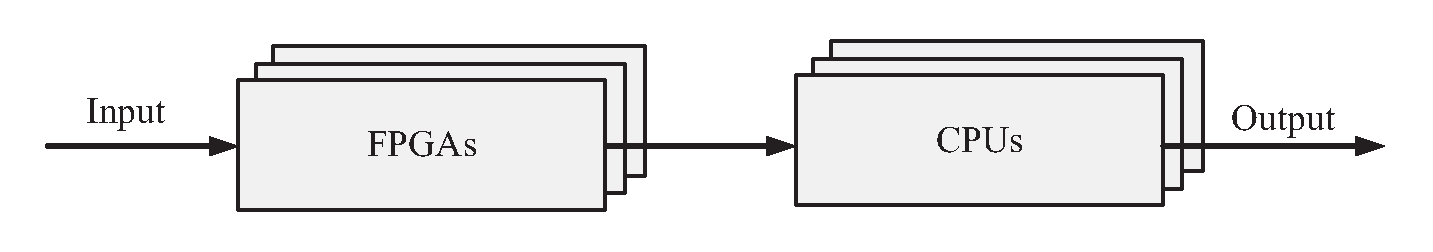
\includegraphics[width=0.7\textwidth]{1_introduction/figures/het_arch1}
	\label{fig:het_arch1}
}
\subfigure[]{
	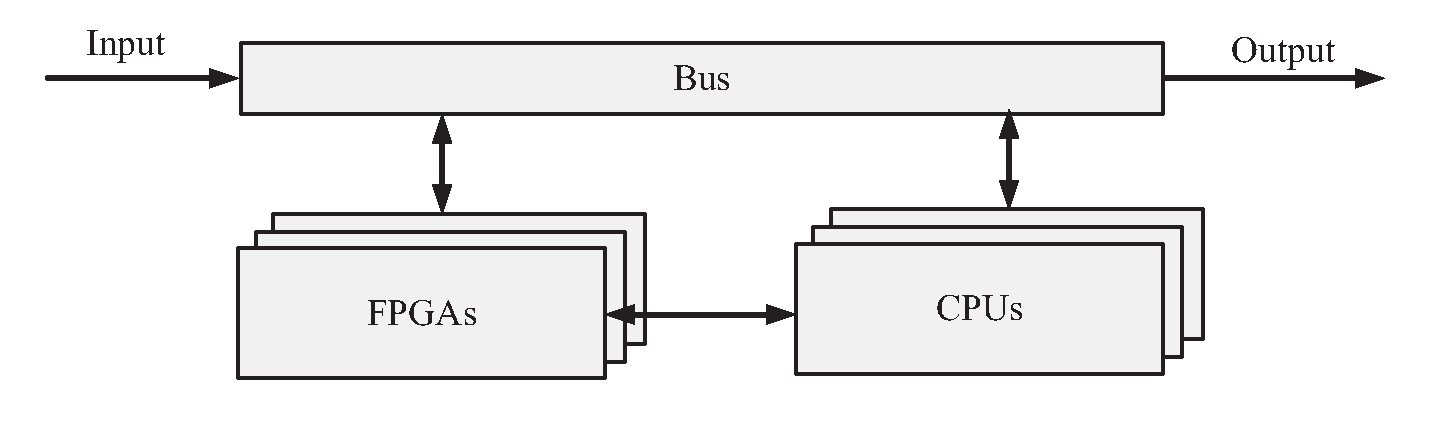
\includegraphics[width=0.7\textwidth]{1_introduction/figures/het_arch2}
	\label{fig:het_arch2}
}
\caption{Illustration of heterogeneous processing topologies: (a) Pre-processing by FPGAs; (b) Co-processing between FPGAs and CPUs.}
\label{fig:het_arch}
\end{figure}

The three subsections that follow offer a brief overview of each contribution and the challenges involved.
More detail explanations are presented in the individual chapters of this thesis.

\subsection{Precision Optimisation of Reconfigurable Data-paths}

The first contribution of this thesis is \textit{precision optimisation approach to maximise real-time performance of reconfigurable systems}.

\glspl{fpga} have abundant fine-grained resources but the clock speeds of \glspl{fpga} are commonly 10 to 30 times slower than \glspl{cpu} and \gls{gpu},
therefore the performance gains in \glspl{fpga} are obtained by designing algorithms such that many independent operations can occur simultaneously.
A crucial step to unleash competitive performance of \glspl{fpga} is to provide massive parallelism and effective use of data.
By employing significant data-path parallelism and deep pipelines where inputs and outputs continually stream through each cycle, hundreds or even thousands of operations are executed on \glspl{fpga} each cycle to outweigh the slow clock frequencies.
However, each data-path requires replication of circuits and deep pipelines need numerous flip-flops, resource usage and bandwidth requirement are often the performance limitation for \gls{fpga} implementations~\cite{stitt11}.

Currently, \glspl{fpga} have the ability to support customisable data-paths of different precisions.
Reduced precision data-paths consume less logic resource and hence allow a higher degree of parallelism.
Using reduced precision also requires lower I/O bandwidth and has higher clock frequencies.
Unfortunately, all the mentioned benefits come with an expense of lower accuracy of results.
There are trade-offs between performance and accuracy in the implementation of data-paths.

Chapter~\ref{ch:precision} describes how reduced precision is applied to reconfigurable systems.
A novel data structure and a memory architecture are developed to support reduced precision data-paths on multiple \glspl{fpga} and to maintain the accuracy of final results by re-computing a small fraction of \gls{fpga} outputs on ~\glspl{cpu}.
This work employs the pre-processing topology (Figure~\ref{fig:het_arch1}), the data-paths on \glspl{fpga} compute and filter most of the data before sending the filtered data to \glspl{cpu} for re-computation.

The proposed methodology is applied to an image-guided surgical robot application which employs the \gls{pq} process.
Functional transformation further optimises the data-path for hardware-friendly implementation.
Implementation in a reconfigurable platform with four \glspl{fpga} shows 58 times speedup over a 12-core \gls{cpu} system, 3 times speedup over a \gls{gpu} system, and 3 times speedup over the same reconfigurable platform without precision optimisation.

\subsection{Run-time Adaptation of System Configuration}

The second contribution of this thesis is \textit{an approach that adapts the reconfigurable systems at run-time for reduced computation workload and energy consumption}.

Power and energy efficiency is becoming a major consideration for ~\gls{hpc} systems.
For example, the Green500 list~\cite{green500} provides a ranking of the energy efficiency of world-wide supercomputers.
\glspl{cpu} are equipped with various technologies to reduce power dissipation~\cite{intelsleep,intelturboboost}.
\glspl{gpu} also have different power modes~\cite{amdpower,nvidiapower}.
As \glspl{fpga} are increasingly being deployed for \gls{hpc}, power dissipation is also a concern when designing \gls{fpga} applications.
Apart from traditional power saving techniques such as clock gating and dynamic frequency/voltage scaling, which exist on other platforms, \glspl{fpga}' run-time reconfigurability could be exploited as an aggressive power saving technique.
The power consumption of an \gls{fpga} depends on the circuit size and the clock frequency.
Larger circuit uses more routing tracks which bring parasitic capacitance,
and higher clock speed increases the switching activity on these routing tracks which causes significant power dissipation.

Chapter~\ref{ch:adaptation} explores an adaptation approach to reduce \gls{fpga}'s energy consumption by run-time reconfiguration.
In particular, \gls{smc} applications are studied as they facilitate adaptation at two different levels.
At algorithmic level, an adaptive \gls{smc} algorithm which adjusts the computation workload at run-time while maintaining the quality of results is proposed.
At system level, run-time reconfigurability of \glspl{fpga} is used to switch the real-time system between computation mode and low-power mode.
Low-power mode lowers the dynamic power by reducing circuit size and clock frequency.
Compared to a non-adaptive and non-reconfigurable system, the proposed approach reduce idle power by 25-34\% and the overall energy consumption by 17-33\%.

This work employs the co-processing topology (Figure~\ref{fig:het_arch2}), the \glspl{fpga} handle the computation which can be fully-pipelined, while the \glspl{cpu} deal with non-sequential data access.

\subsection{Design Flow for Domain-specific Reconfigurable Applications}

The final contribution of this thesis is \textit{the development of a design flow that reduce the development effort of real-time applications on reconfigurable systems}.

Although \glspl{fpga} show promising performance advantage for high-performance real-time systems, \gls{fpga} accelerators have not yet been accepted by mainstream application designers~\cite{stitt11}.
Low productivity and long design time have long been the main barriers to bring \glspl{fpga} to more wide-spread usage.
The design complexity of \gls{fpga} applications far exceeds that of \glspl{cpu} and \glspl{gpu}, and hence raises development cost and deter user acceptance.
Traditionally, \gls{fpga} applications are developed using \glspl{hdl} which is timing-consuming and requires digital design expertise and knowledge of low-level device details that are not common to mainstream designers.
In addition, designers have to perform numerical analysis to determine an appropriate precision in order to achieve an \gls{fpga}'s full potential.
It is because \glspl{fpga} often achieve order of magnitude improvements when using fixed-point, integer, or bit-level operations.
This process significantly increases design time.
Another productivity bottleneck is lengthy compilation times due to the complexity of placement and routing.
Common software design practices based on rapid compilation are no longer feasible for reconfigurable system design.

In Chapter~\ref{ch:tool}, a design flow is proposed to address the above mentioned challenge.
This chapter extends the \gls{smc} reconfigurable system described in Chapter~\ref{ch:adaptation} and focuses on making the system parametrisable for a wide variety of \gls{smc} applications.
In other words, it makes Chapter~\ref{ch:adaptation}'s reconfigurable system easier and more accessible to designers, especially those lack hardware design experience.
Through templating the \gls{smc} structure, the proposed design flow enables efficient mapping of applications to multiple \glspl{fpga}.
To reduce design space exploration effort, a machine learning algorithm based on surrogate modelling is used to tune design parameters that are crucial to the performance and solution quality.
The design flow demonstrates its capability of producing reconfigurable implementations for a range of \gls{smc} applications that have significant improvement in speed and in energy efficiency over optimised \gls{cpu} and \gls{gpu} implementations.


\section{Thesis Organisation}

\textbf{Chapter~\ref{ch:background}} offers a detailed background on reconfigurable architectures and systems, design flow which includes synthesis tools and programming languages, and the applications of reconfigurable technologies on real-time systems.
The first contribution of this thesis is described in \textbf{Chapter~\ref{ch:precision}}, which demonstrates how precision optimisation is applied to reconfigurable real-time systems.
The proposed methodology is applied to an application in imaged-guided surgical robot based on \gls{pq} process. 
\textbf{Chapter~\ref{ch:adaptation}} presents the second contribution of this thesis, which describes using run-time reconfigurability of \glspl{fpga} to adapt real-time systems for reduced power and energy consumption.
The final contribution of this thesis can be found \textbf{Chapter~\ref{ch:tool}}, which describes a design flow for automatically generating efficient implementation of reconfigurable designs.
Lastly, Chapter~\ref{ch:conclusion} concludes this thesis, and presents the outstanding challenges that remain.

\begin{figure}[ht]
\begin{center}
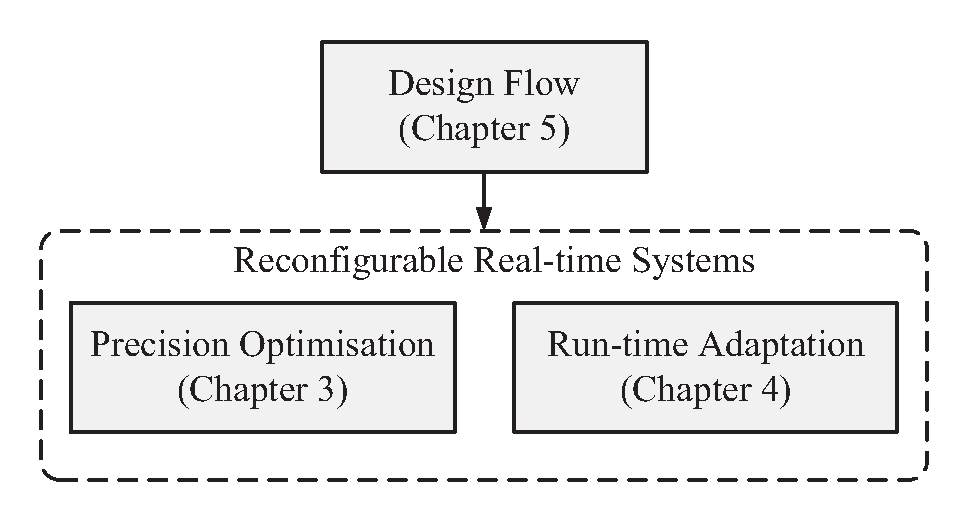
\includegraphics[width=0.7\textwidth]{1_introduction/figures/organisation}
\end{center}
\caption{Thesis organisation}
\label{fig:intro_organisation}
\end{figure}

Parts of this thesis have been published in~\cite{chau13fpt,chau13arc,chau14trets,chau14fccm}.
During the course of this work, several related papers were also published.
Papers~\cite{chau13acm,eele13cdc,eele13gnc} show the details of accelerating air traffic management systems, which is one of the \gls{smc} applications being studied in Chapter~\ref{ch:tool}.
Paper~\cite{kurek14fccm} presents details of surrogate modelling that enable machine learning approach in Chapter~\ref{ch:tool}.
Papers~\cite{chau12fpl,niu13fccm} present an initial work about adaptive \gls{smc} method, which lead to the proposal in Chapter~\ref{ch:adaptation}.
Paper~\cite{chau12heart} aims to provide a simple benchmarking platform for real-time systems.
Due to page limitation, neither of these contributions are described in this thesis.

\section{Statement of Originality}

I declare that this thesis was composed by myself, and that the work it presents is my own, except where otherwise stated.

